\section*{Introduction}
\addtocontents{toc}{\protect\setcounter{tocdepth}{0}}
The problem of time series prediction (and related regressional tasks) have been a long standing subject of high interest in many disciplines of science and mathematics. The problem itself is fairly straight forward, given a data set of $n$ observations $\calD = \left\{ \left( x_i , y_i \right) \right\}_{i=1}^{n}$, where each input $x_i \in \RR_{>0}$ is a time value and $y_i \in \RR$ is a that acts a function of time, the question then is how do we go about predicting a value $y_{\star}$ for the modeled phenomena at time $x_{\star}$? With computing power becoming ever more affordable and advanced, many have taken to Machine Learning (ML) to develope sophisticated models to address the problem of developing accurate time series predictors. ML, broadly speaking, is any class of heuristic algorithm that attempts to refine and develope functionality by learning through some form of input. The idea of ML is founded on the idea that any form of task learning is done through sensory input taken from the surrounding environment. More formally speaking, in ML we are trying to develope a function $f : X \to Y$ for some input set $X$ and observation set $Y$ were the outputs of $f$ closely align to actual observations. A model will attempt to make accurate prediction using some simplified formulation of the world required for the task. The distribution corresponding to the probability of a prediction within the context of the "state of the world" is referred to as the {\it likelihood}. The uncertainty within the likelihood stems from the predictive limits of the model. These limitation usually arise as a consequence of selecting a model too simple or complex for the task. The "state of the world" is sometimes internally captured by the model as a set of mutable parameters $\bm{\theta}$. The process of taking observations and using them to form predictions is called {\it inference} which, in some sense, is synonymous with learning.

ML can be applied the problem of time series prediction in a fairly straight forward manner, by simply teaching a ML algorithm $\calM$ the time series data set $\calD$ to hopefully produce a function $f$ that serves as a good approximant for event prediction. In this thesis we shall focus on particular class of ML algorithms called Baysian ML models which, unsurprisingly, makes use of Bayesian statistics to drive inference.

In Baysian models a {\it prior} distribution is used to represent the uncertainty of the current state of the model before any observations are made. The model can then be updated once data is observed by using the likelihood to update the state of the model to give a {\it posterior} distribution which represents the reduced uncertainty after "teaching" the model with these new observations. Methods of "teaching" a model how to behave using a new set of observations sometimes involves the use of a {\it loss function} $L$ is used to aid us in deciding what action $a$ should be taken in changing the state of the model to best minimize uncertainty. The best action, roughly speaking, can be evaluated as
\begin{equation*}
    a_{\star} =  \argmin_{a} \int L \left( y_{\star} , a \right) p \left( y_{\star} \mid \bm{x}_{\star}, \bm{X}, \bm{y} \right) \; d y_{\star}.
\end{equation*}
Interestingly, the best action does not rely so much on the model internalized parameters of the structure of the model itself but more so the predictive distribution $p \left( y_{\star} \mid \bm{x}_{\star}, \bm{X}, \bm{y} \right)$. This key insight has spawned a class of ML algorithms that focus on infering the function $f$ directly by computing $p \left( f \mid \calD \right)$ instead of finding optimal internal parameters using $p \left( \bm{\theta} \mid \calD \right)$. Models that perform inference in this manner as called {\it non-parameteric} models. Within the {\it non-parameteric} model paradigm, the predictive distribution can be expressed as
\begin{equation*}
    p \left( y_{\star} \mid x_{\star} , \bm{X} , \bm{y} \right) = \int p \left( y_{\star} \mid f , x_{\star} \right) p \left( f \mid \bm{X} , \bm{y} \right) \; df
\end{equation*}
and once new data is observed the posterior can be updated using Baye's rule
\begin{equation*}
    \text{posterior} = \frac{\text{likelihood} \times \text{prior}}{\text{marginal likelihood}}, \qquad p \left( \bm{f} , f_{\star} \mid \bm{y} \right) = \frac{p \left( \bm{y} \mid \bm{f} \right) p \left( \bm{f} , f_{\star} \right) }{p \left( \bm{y} \right)}.
\end{equation*}
This thesis will focus on a particular non-parameteric Bayesian ML model called Gaussian processes (GP). The over arching idea of GPs is to define a prior to every possible function mapping from $X$ to $Y$. On the surface, this does not seem computationally tractable as we would seemingly need to check through an uncountable infinite number of mappings. It turns out, computation can be completed given we are only seeking predictions at a finite number of points using a finite number of observations. GPs occupy a special place within the realm of ML since they account for uncertainty in a principled way, relatively simple to implement and are highly modular allowing them to easily be incorporated into a larger systems. It is no surprise that while other kernel methods are still overshadowed by their neural network cousins, GPs have made a quiet comeback in the ML community.

To highlight a particular GP success story, a team of agriculturalists lead by Andries Potgieter are currently investigating how ML can be used to inform farmers on the best time to plant various crops to minimize crop loss from environmental stresses; such as frost and plant diseases. This involves analysing crop growth from previous seasons to forecast when certain phenological stages in the crops development of the current yield. This problem is readily converted into a time series problem. Originally, Andries' team surveyed a number of different parameteric models to provide this forecasting. However, the parameteric models we serverely limited in their ability to inform when key phenological stages would take place. They then moved onto using GPs which they found could produce much higher resolution predictions from which they could infer a far richer phenological timeline. A comparision of using GPs over other parameteric models is shown in Figure \ref{fig: GP_motivate_wheat}.
\begin{figure}[h]
    \centering
    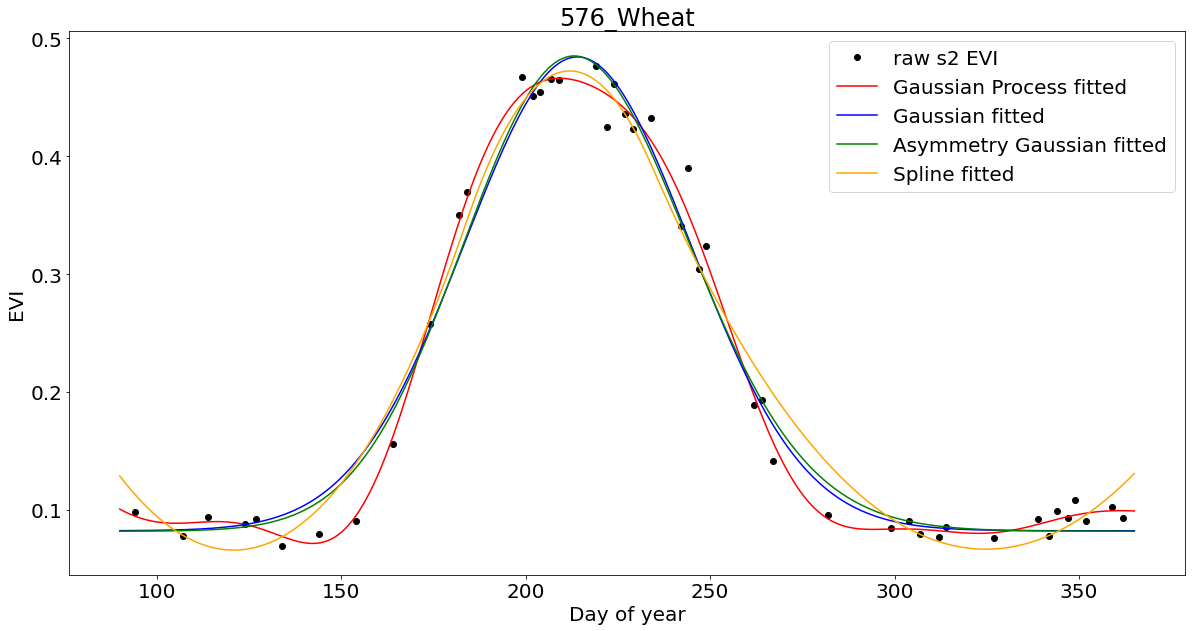
\includegraphics[scale=0.3]{img/yan_wheat_GPR_plot.png}
    \caption{Andries' team found that GPs where superior in terms of predicting a phenological timeline for a number of common seasonal crops over other parameteric models.}
    \label{fig: GP_motivate_wheat}
\end{figure}
Andries' team found that the only draw back to using GPs was the lengthy run time required to create predictions and fears that as more data is collected each season this would only exacerbate the issue. This is a common problem shared by anyone wanting to use GPs. Due to their unwieldy $\calO \left( n^3 \right)$ runtime, where $n$ is the number of observations,  GPs become impractical to apply on datasets with $n > 10^5$. The goal of this thesis is to explore various avenues one can take to replace some of the more intense calculations with computational more efficient approximations without sacrificing a great deal of precision.

Chapter \ref{Chapter1} will give a more mathematical treatment of GPs starting from the ground up by first giving a review of some essential material from functional analysis and then motivating the theory behind GPs before finally ending with a concrete algorithm for GP regression and classification. In chapter FIX and \ref{Chapter3} we shall look at techniques for approximating a large matrix that essentially provides information on how similar each observation is from one other. Chapter \ref{Chapter4} then gives alternative methods for solving linear systems which is an essential component required for GP algorithm to work.

\newpage
\addtocontents{toc}{\protect\setcounter{tocdepth}{2}}
%%%%%%%%%%%%%%%%%%%%%%%%%%%%%%%%%%%%%%%%%%%%%%%%%%%%%%%%%%%%%%%%%%%%%%%%%%%%%%%